% ------------------------------------------------------------------------
%%%%% Start of preamble %%%%%
% ------------------------------------------------------------------------

%%%%---------What kind of document  and what size--------------------------------------
\documentclass[12pt]{article}

%%%MY: Other possible document: article, report, amsart, thesis, book,etc.


%%%%---------Packages to load which give you useful commands---------------------------------
\usepackage{graphicx} %to include pictures and figures
\usepackage{amssymb, amsmath, amsthm} %to include standard American Mathematical Society math symbols and fonts
\usepackage{fontenc} %to be able to include more font
\usepackage{amscd,latexsym,amsfonts,amstext,amsbsy} %more AMS fonts and options
\usepackage{euscript} %for european script
\usepackage{enumerate} %for automatic enumeration of equations, items, etc.
\usepackage{color}  %to change the color of a text.
\usepackage{physics}
\usepackage[latin1]{inputenc}
\usepackage{tikz}
\usepackage{mathrsfs}
\usetikzlibrary{shapes,arrows}
\usepackage{multicol}
\usepackage{color,soul}

\textwidth = 16 cm
\textheight = 24 cm
\oddsidemargin = 0.0 cm
\evensidemargin = 0.0 cm
\topmargin = -2 cm
%\headheight = 0.0 in
%\headsep = 0.0 in
\parskip = 0.2in
\parindent = 0.0in


 \newtheorem{theorem}{Theorem}
  \newtheorem{problem}[theorem]{Problem}
   \newtheorem{exercise}[theorem]{Exercise}
 \newtheorem{corollary}[theorem]{Corollary}
 \newtheorem{lemma}[theorem]{Lemma}
 \newtheorem{proposition}[theorem]{Proposition}
 \newtheorem{proporties}[theorem]{Proporties}
 \newtheorem{definition}[theorem]{Definition}
  \newtheorem{definitions}[theorem]{Definitions}
  \newtheorem{example}[theorem]{Example}
 \newtheorem{remark}[theorem]{Remark}
 


\begin{document}
\textbf{Heroin Model} \\
Tricia Phillips \\
\today \\

\textbf{Background} \\ \\
The misuse of opioids, a drug class including prescription pain relievers and the illegal drug heroin, is rampant in today's society. The opioid crisis was declared a public health emergency in October 2017 by the United States Department of Health and Human Sciences [15]. In 2016, there were 11.8 million opioid misusers 12 years of age or older with 948,000 of these being heroin users [10]. In addition, there was an estimated 13,219 heroin deaths in 2016, a more than six-fold increase from the year 2002 [7]. This, in part, is due to the recent trend of lacing heroin with fentanyl, a surgical-grade opioid that is up to fifty times more potent than heroin alone, and therefore, users are unaware of the purity of the heroin they obtain [9,12]. 

Prescription pain relievers are misused for a variety of reasons with the most prominent being to relieve physical pain, to feel good or get high and to relax or relieve tension. Individuals that misuse prescription opioids mostly obtain them from friends/relatives or from a healthcare provider, with misuse defined as taking the prescription at a higher dose or more frequently than prescribed, or taking someone else's medication [10]. 

To address this apparent problem in today's society, we have formulated a population level model to investigate the dynamics among individuals taking prescription opioids, addicted to opioids, using heroin and recovering from opioid and/or heroin addiction. Opioids are of no shortage in society today. The number of prescriptions that pharmacies distributed in 2011 was almost triple that of 1991 and there is a higher availability of heroin in recent years at a lower cost than alternative opioids [14]. This leads some individuals to start heroin, and in fact, 80\% of heroin users used prescription opioids before their heroin use [32]. We aim to find ways to optimally treat pain with prescriptions while reducing opioid addiction and heroin use. The motivation for this model came from a previous model focusing on opioid addicts through prescriptions or via the black market; the purpose of formulating a separate model is to be able to understand the more complicated dynamics that arise among opioid addiction with the addition of heroin use [1].  

\textbf{Model Formulation} \\ \\
Our model consists of five subgroups of the (national) population: 

1. Susceptibles ($S$): This portion of the population consists of individuals who are not taking prescription opioids of any kind, nor are using heroin. \\ \\
2. Prescription opioid users ($P$): This class of individuals consists of individuals who are prescribed opioids by a health care provider and take the opioids as recommended by their doctor, so they are not considered addicted. \\ \\
3. Opioid addicts ($A$): This group of individuals are addicted to opioids or are dependent on opioids. Although the opioid class of drug includes heroin, here we will take opioids to mean non-heroin.  \\ \\
4. Heroin users ($H$): This class is composed of individuals who use heroin, which is implicitly understood to be addictive. \\ \\
5. Individuals in treatment/rehabilitation ($R$): This class consists of individuals undergoing treatment for their addiction to opioids and/or heroin. 

We denote the initial conditions as
$S(0)=S_{0}$, $P(0)=P_{0}$, $A(0)=A_{0}$, $H(0)=H_{0}$, and $R(0)=R_{0}$, and we assume all of these values are positive. From data, the initial values for each of the classes are the following proportions of the entire population, and therefore are dimension-less: $S_{0}=0.6068$, $P_{0}=0.38$, $A_{0}=0.0062$, $H_{0}=0.0026$, and $R_{0}=0.0044$, where $R_0$ is calculated to be the sum of opioid addicts entered into treatment (772,000) and heroin users entered into treatment (618,000) in 2014, divided by the total population of 319 million in 2014  [4,21,14,23].  \\ \\
Here, we present our ordinary differential equation model: 
\[\dv{S}{t} = -\alpha S - \beta (1- \xi) SA  -\beta \xi SP- \theta_{1} SH +\epsilon P +\delta R +\mu (P+R) + (\mu+\mu_{A})A + (\mu+\mu_{H}) H \quad (1)\] 
\[\dv{P}{t} = \alpha S - \epsilon P  - \gamma P - \theta_{2}PH- \mu P    \quad(2)\]
\[\dv{A}{t} = \gamma P + \sigma_{A} R +\beta (1- \xi) SA  +\beta \xi SP -\zeta A - \theta_{3}AH-(\mu + \mu_{A})A   \quad (3)\]
\[\dv{H}{t} = \theta_{1}SH+\theta_{2}PH+\theta_{3}AH + \sigma_{H}R-\nu H-(\mu+\mu_{H})H  \quad (4)\]
\[\dv{R}{t} = \zeta A +\nu H -\delta R -\sigma_{A}R-\sigma_{H}R -\mu R\quad(5).\]


The parameters involved in this model represent transition rates from one class to another; specifically: 
\begin{itemize}
\item $\alpha$: rate at which individuals are prescribed opioids (1/year)
\item $\beta$ : rate of becoming addicted to opioids by some means other than prescription (1/year)
\item $\beta(1-\xi)$: rate of becoming addicted to opioids by black market drugs or interaction with other addicts (1/year, dimension-less)
\item $\beta \xi$ : proportion of the susceptible population that obtains extra prescription opioids and becomes addicted  (1/year, dimension-less)
\item $\theta_1$: rate at which the susceptible population becomes addicted to heroin by black market availability or interaction with other heroin users  (1/year)
\item $\epsilon$: rate at which people come back to the susceptible class after being prescribed opioids and did not develop an addiction (1/year) 
\item $\delta$: rate at which both opioid and heroin addicts enter back into the susceptible class after successfully finishing treatment (1/year)
\item $\mu$: natural death rate (1/year)
\item $\mu_A$: enhanced death rate for opioid addicts; overdose rate which results in death (1/year)
\item $\mu_H$: enhanced death rate for heroin addicts; overdose rate which results in death (1/year)
\item $\gamma$: rate at which prescribed opioid users become addicted to opioids (1/year)
\item $\theta_2$: rate at which prescribed opioid users become addicted to heroin (1/year)
\item $\sigma_A$: rate at which individuals transition from treatment into the opioid addicted class (note: not considered relapse because do not know where individuals came from originally) (1/year)
\item $\zeta$: rate at which addicted opioid users enter treatment/rehabilitation (1/year)
\item $\theta_3$: rate at which the opioid addicted population becomes addicted to heroin  (1/year)
\item$\sigma_H$: rate at which individuals transition from treatment into the heroin addicted class (note: not considered relapse because do not know where individuals came from originally) (1/year)
\item $\nu$: rate at which heroin users enter treatment/rehabilitation 
\end{itemize}

We note that although sellers are not directly involved in the model nor have to be addicts themselves, addicted individuals act as a proxy for sellers of the drug and general availability of the drug, whether it is opioids or heroin. This is because the higher number of addicted individuals there are, the more sellers there needs to be which results in an increased exposure to the drug and therefore, increased chance of addiction.  
This compartmental model can be represented by the following flow diagram with each arrow representing either the transition rate between one class to another or death: 

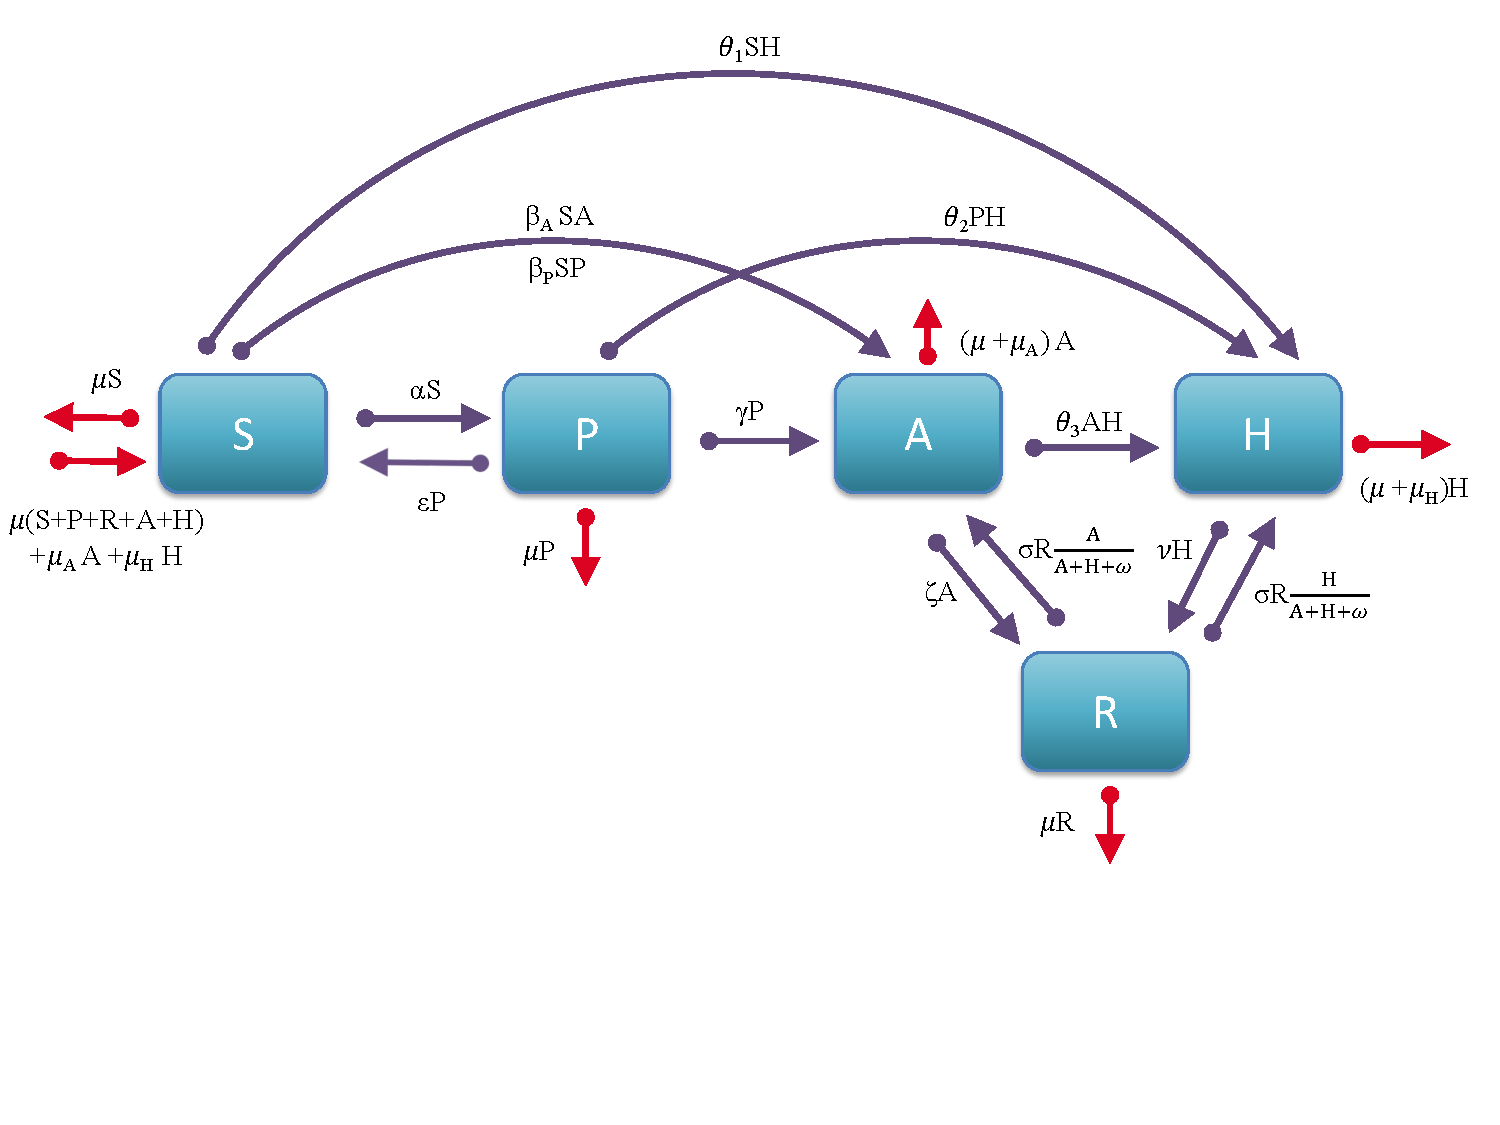
\includegraphics[scale=0.6]{heroin_schematic.pdf}

Initial conditions were estimated from the literature from the year 2015 and 2016. The number of prescribed, non-addicted opioid users in 2015 was estimated to be 91.8 million adults, and this is approximately 38\% of the population [4]. The number of addicted opioid users was estimated to be 2 million, which is .59\% of the 2016 total population of 324 million [21]. The number of heroin users in 2015 was estimated to be 828,000 people which is .26\% of the population. Finally, 772000 opioid users and 618000 heroin users entered treatment in the year 2014 which is .44\% of the 2014 total population of about 319,000,000 [14]. This leaves the remaining 60\% of the population as susceptible. 

The parameters for our model were estimated from the literature on opioids and heroin. 

In 2015, individuals were prescribed opioids at a rate of 20.7 people out of 100, causing $\alpha=0.207$ [20].

Need to fix$--$$>$It is estimated that eighty percent of those who use heroin misused prescription opioids in the past; we will make the assumption that individuals were addicted to opioids previously in order to estimate some parameters [30]. In 2015, there were 828,000 heroin users, meaning that 662,400 of them were addicted to prescription opioids [14]. Making the assumption that the chance of becoming a heroin user is equal among susceptible individuals and prescription opioid users, we will split the remaining 165,600 individuals into these two groups. In that case, 82,800 susceptible individuals becoming a heroin user out of a total population of 321,000,000 results in $\theta_{1}=0.0003$, and similarly for prescription opioids users, leading $\theta_{2}$ to be the same value. 


In 2011, a study was performed that resulted in a 90\% relapse rate to opioid use within one year after treatment ending, so that $\sigma_{A}=0.9$ [19]. 

We assume that individuals who go to treatment to deal with their addiction to opioids can only fall back into the opioid addiction class, and those who enter for heroin use only fall back into the heroin class. 

Based on $\sigma_{A}=0.9$ and $\sigma_{H}=$, this implied  $\delta=0.1$ + success from heroin , those who successfully ended their addiction to opioids [28, other ]. 

The death rate $\mu$ for the total population in 2015 was 2,712,630 people, or 0.84\%, which we make note includes opioid and heroin related deaths, as well [24]. 

The opioid overdose rate in 2015 was 4 out of 100,000 individuals, resulting in $\mu_A=.00004$, and similarly for $\mu_H$ [25]. 

Prescription opioid users become dependent on opioids at a rate of 26\%, resulting in $\gamma=0.26$ and $\epsilon=0.74$ [28].

Four percent of prescription opioid users start using heroin, leading to $\theta_3=.04$ and heroin users enter treatment at a rate of 15\% so that $\nu=.15$ [14]. 

 \textbf{Proof of existence of solution to ODE system} \\
Will show existence of solution to my ODE system. 


\textbf{Proof of non-negative initial conditions guaranteeing non-negative solutions} \\
 Will show that starting with positive initial conditions, will stay positive for all time.

 
 
\textbf{Addiction-Free Equilibrium} 

To find the addiction-free equilibrium, we set equations (1)-(5) equal to zero and require that $A=H=R=0$. We are left with the system: \\
\[0=-\alpha S^* -\beta \xi S^* P^* + \epsilon P^* +\mu P^* \quad\]
\[0=\alpha S^* - \epsilon P^* -\gamma P^* - \mu P^* \quad\]
\[0=\gamma P^* + \beta \xi S^* P^*.   \quad\]



If $P^*=0$, then the only solution is $S^*=P^*=H^*=R^*=0$. Thus, we will assume $P^* \neq 0. $ This forces $\gamma + \beta \xi S^* =0$ and since all of our parameters and variables are non-negative, then it must be $\gamma=0$ and either $\beta=0$ or $\xi=0$. Under the assumption that $\gamma=0=\xi$ to ensure the existence of our addiction-free equilibrium and that $1=S+P+A+H+R$, we calculate the addiction-free equilibrium to be: \\

\[S^*=\frac{\epsilon + \mu}{\alpha + \epsilon +\mu}\quad\]
\[P^*=\frac{\alpha}{\alpha + \epsilon +\mu}\quad\]
\[A^*=0\quad\]
\[H^*=0\quad\]
\[R^*=0\quad\] 

Note that enforcing $P^* \neq 0$ implies that $\alpha \neq 0$, as well.

\textbf{Basic Reproduction Number, \textbf{$\mathscr{R}_0$}}

The basic reproduction number, denoted $\mathscr{R}_0$, is a term used in epidemiological models that gives the expected number of secondary disease cases that result from the introduction of a disease to a susceptible population. The value of $\mathscr{R}_0$ represents how successful the spread of the disease is expected to be; if $\mathscr{R}_0 < 1$, then the disease is expected to die out and the disease-free equilibrium will be locally stable; conversely, if $\mathscr{R}_0 >1$, then the disease is expected to spread and the disease-free equilibrium will be unstable [11]. This idea may be applied to the context of our model since addiction to opioids and use of heroin may be viewed similarly to that of a disease. That is, opioid addiction and heroin use/addiction can "spread," meaning that susceptible individuals who interact with opioid addicts and heroin users have the potential of becoming addicts themselves. The disease compartments are those that contain infected individuals, or in our case, addicts [11]. Our model incorporates three addiction compartments, A, H, and R, since these all consist of opioid and/or heroin addicted individuals and these subpopulations are put into a vector, $x= {[A\quad H\quad R]}^{T}$. Then, in general, the differential equations of the $n$ disease compartments, $x_i'$, may be written as: 

\[{x_i'} = \mathscr{F}_{i} (x,y)-\mathscr{V}_i (x,y),\quad i=1,...,n\] 

where $\mathscr{F}_{i}$ represents the rate that secondary infections contribute to disease compartment $i$ and $\mathscr{V}_{i}$ represents the rate at which the disease compartment $i$ is decreased by means of death, recovery and progression of the disease [11]. 



For the purposes of calculating $\mathscr{R}_0$, we will assume $\gamma =0$ and $\xi =0$ (thus, $\beta \neq 0$) in order to ensure the existence of the addiction-free equilibrium. This results in the following system:
\[\dv{S}{t} = -\alpha S - \beta SA  - \theta_{1} SH +\epsilon P +\delta R +\mu (P+R) + (\mu+\mu_{A})A + (\mu+\mu_{H}) H \quad \] 
\[\dv{P}{t} = \alpha S - \epsilon P  - \theta_{2}PH- \mu P    \quad\]
\[\dv{A}{t} = \sigma_{A} R +\beta SA  -\zeta A - \theta_{3}AH-(\mu + \mu_{A})A   \quad\]
\[\dv{H}{t} = \theta_{1}SH+\theta_{2}PH+\theta_{3}AH + \sigma_{H}R-\nu H-(\mu+\mu_{H})H  \quad\]
\[\dv{R}{t} = \zeta A +\nu H -\delta R -\sigma_{A}R-\sigma_{H}R -\mu R.\quad\]

Thus, under the assumption that A, H and R are the disease, or addicted, compartments and abiding by the parameter restrictions stated above, the assumptions of the Next Generation Method are satisfied for matrices $\mathscr{F}$ and $\mathscr{V}$ formulated here:

\begin{center}
$\mathscr{F}=$
$ \begin{pmatrix}

0 \\
0 \\
\beta SA \\
\theta_{1}SH+\theta_{2}PH \\
0
\end{pmatrix}$



$\mathscr{V}=$
$ \begin{pmatrix}

\alpha S + \beta SA+\theta_{1}SH-\epsilon P-\delta R-\mu(P+R+A+H)-\mu_{A}A-\mu_{H}H \\
-\alpha S+\epsilon P +\theta_{2}PH +\mu P \\
-\sigma_{A}R+\zeta A+\theta_{3} AH + (\mu +\mu_{A})A \\
-\theta_{3}AH-\sigma_{H}R+\nu H +(\mu +\mu_{H}) H \\
-\zeta A -\nu H +\delta R +\sigma_{A}R +\sigma_{H}R +\mu R\\
\end{pmatrix}$.
\end{center}

Taking $F=\frac{\partial \mathscr{F}_i}{\partial x_j} (0, y_0)$ and $V=\frac{\partial \mathscr{V}_i}{\partial x_j} (0, y_0)$, where (0, $y_{0}$) $=(\frac{\epsilon + \mu}{\alpha + \epsilon +\mu},\frac{\alpha}{\alpha + \epsilon +\mu},0,0,0)$ is the addiction-free equilibrium, we calculated the following [11]: 



\begin{center}
$F=$
$ \begin{pmatrix}

\beta S^* &  0  & 0 \\
0 & \theta_1 S^* +\theta_2 P^* & 0\\
0  &   0 & 0\\
\end{pmatrix}$



$V=$
$ \begin{pmatrix}

\zeta +\mu +\mu_A &  0  & -\sigma_A \\
0 &  \nu+\mu+\mu_H & -\sigma_H\\
-\zeta& -\nu  & \delta + \sigma_A + \sigma_H + \mu\\

\end{pmatrix}$.
\end{center}

The eigenvalues of $FV^{-1}$ are calculated to be: 
\begin{center}
$\sigma (FV^{-1}) = \{0, \frac{(r+s)-\sqrt{(r-s)^2+4\beta S^* z  \sigma_A \zeta \sigma_H \nu}}{2det(V)} 
, \frac{(r+s)+\sqrt{(r-s)^2+4\beta S^* z  \sigma_A \zeta \sigma_H \nu}}{2det(V)} 
\}$
\end{center}

$\mathscr{R}_0$ may then be determined as the spectral radius of $FV^{-1}$:
\begin{center}
$\mathscr{R}_0=$ $\frac{(r+s)+\sqrt{(r-s)^2+4\beta S^* z  \sigma_A \zeta \sigma_H \nu}}{2det(V)} $
\end{center}
where $a=\zeta +\mu + \mu_A$, $b=\nu + \mu + \mu_H$, $c=\delta + \sigma_A + \sigma_H +\mu$, $z=\theta_1 S^* + \theta_2 P^*$, $ r=\beta S^* (bc-\sigma_H \nu), s=z(ac-\sigma_{A} \zeta)$, and $det(V)=a(bc-\sigma_H\nu)-\sigma_A\zeta b$.

This value is the spectral radius since it is the largest eigenvalue greater than 0. We can see this by first noting that the radicand $(r-s)^2+4\beta S^* z  \sigma_{A} \zeta \sigma_{H} \nu$ is positive, since all parameters are positive. In addition, $r$ is positive because in the multiplication of $bc=\delta \mu + \delta \nu+ \delta \mu_{H}+ \mu^{2} + \mu \nu+ \mu \mu_{H} + \mu \sigma_{A} + \mu \sigma_{H}+ \nu \sigma_{A}+$ \hl{$ \sigma_{H} \nu $} $+ \mu_{H}\sigma_{A}+\mu_{H}\sigma_{H}$, all terms are positive and the highlighted term cancels with $-\sigma_{H} \nu$, leaving only a positive sum. Multiplying by $\beta S^*$, the resulting value $r$ is positive. Similarly, $s$ is positive because in the multiplication of $ac=\delta \mu_{A} + \delta \mu + \delta \zeta + \mu_{A} \mu+ \mu_{A} \sigma_{A}+\mu_{A} \sigma_{H} +\mu^{2} +\mu \zeta+ \mu \sigma_{A}+\mu \sigma_{H}+$ \hl{$\sigma_{A} \zeta$} $+ \zeta \sigma_{H}$, all terms are positive and the highlighted term cancels with $-\sigma_{A} \zeta$, again resulting in a sum of only positive terms. Multiplied against positive value $z$, this results in $s$ being positive. Finally, the expansion of $det(V)$ is positive. This is because $bc$ is a positive sum containing a term that cancels with $-\sigma_{H} \nu$ as described above and $ac$ shown above contains the term $\sigma_{A} \zeta$ which multiplied with b cancels with $-\sigma_A\zeta b,$ thus resulting in a positive determinant. 

Increasing $\beta$ (the rate of addiction via non-prescription means), $\theta_1$ (the rate of heroin addiction of the susceptible population), and $\theta_2$ (the rate of heroin addiction of the prescribed population), all increase $\mathscr{R}_0$ since these parameters only appear in the numerator of $\mathscr{R}_0$, specifically within the $r$, $z$, and $s$ terms. 

\textbf{Sensitivity Analysis} 

In order to explore the sensitivity of each of the population classes to each of the parameters, we implemented Sobol sensitivity analysis in which the Saltelli sampler is utilized to generate N(2D+2) parameter samples where N$=$FILL IN is the number of sample points and D=16, the number of parameters in the model for a total of FILL IN samples [16]. 
Saltelli are the statistically good points chosen in the parameter space to test and records S, P, A, H and R at the final time (t=10 years) for the parameter choices. Samples N points from the problem and returns a matrix of parameter values. 
%Think about why N(2D+2) and why N(D+2) for taking out second order interactions. 

Both $\mu_{A}$ and $\mu_{H}$ were restricted to the domain $[0,0.1]$ with the remaining parameters ranging on the entire domain $[0,1]$. For first-order indices, only one parameter is varied and the rest are held constant; for second-order indices, two parameters are varied and the rest are held constant; and for total-order indices, every combination of parameters is varied, from a single parameter varying alone to all higher-order interactions between parameters. The length of the colored bars, with each color representing a specific class, measures the contribution of a certain parameter to the variance of each of the classes in the model. The longer the colored bar, the higher the effect the parameter has on that class of individuals. We are able to retrieve the confidence intervals on the sensitivity of each of the populations to a respective change in the parameter(s) for first order changes, second order changes and total order changes. \\

%Add in sensitivity analysis results and confidence interval information once converges 
%Takes the mean from the last 100 (or 10 for the case of t=10) time steps. (I thought final time??) \\
%Total --take average of all interactions for plots?? \\
%Need to scale sensitivities of muA and muH based on their domain $[0,0.1]$??






\pagebreak


%\textbf{References}

%$[1]$ On Modeling the Opioid Epidemic -will cite in future \\
%$[2]$ A Comparison of Heroin Epidemic Models \\
%$[3]$ Caldwell, Wendy K., et al. "Substance Abuse via Legally Prescribed Drugs: The Case of Vicodin in the United States." 2013. \\
%$[4]$ Han B, Compton WM, Blanco C, Crane E, Lee J, Jones CM. Prescription Opioid Use, Misuse, and Use Disorders in U.S. Adults: 2015 National Survey on Drug Use and Health. Ann Intern Med. 2017;167:293-301. doi: 10.7326/M17-0865 \\
%$[5]$  Jennifer S. Potter, Elise N. Marino, Maureen P. Hillhouse, Suzanne Nielsen, Katharina Wiest, Catherine P. Canamar, Judith A. Martin, Alfonso Ang, Rachael Baker, Andrew J. Saxon, and Walter Ling
%Journal of Studies on Alcohol and Drugs 2013 74:4, 605-613 \\
%$[6]$ The Prescription Opioid Addiction Treatment Study: What have we learned Weiss, Roger D. et al. Drug \& Alcohol Dependence , Volume 173 , S48 - S54\\
%$[7]$ https://www.samhsa.gov/sites/default/files/topics/data\_outcomes\_quality/nsduh-ppt-09-2017.pdf \\
%$[8]$ https://www.samhsa.gov/sites/default/files/sites/default/files/2016\_ffr\_1\_slideshow\_v5.pdf \\ 
%$[9]$ FILL IN with another fentanyl source\\
%$[10]$ https://www.samhsa.gov/data/sites/default/files/NSDUH-FFR1-2016/NSDUH-FFR1-2016.pdf \\
%$[11]$ Van den Driessche, P., and James Watmough. "Further Notes on the Basic Reproduction Number ." pp. 159-178. \\
%$[12]$ https://www.drugabuse.gov/about-nida/legislative-activities/testimony-to-congress/2016/americas-addiction-to-opioids-heroin-prescription-drug-abuse\#\_ftn2 \\
%$[13]$ https://www.samhsa.gov/data/sites/default/files/2010\_Treatment\_Episode\_Data\_Set\_National/2010\_Treatment\_Episode\_Data\_Set\_National.html\#Fig23 \\
%$[14]$ https://d14rmgtrwzf5a.cloudfront.net/sites/default/files/19774-prescription-opioids-and-heroin.pdf \\
%$[15]$ https://www.hhs.gov/about/news/2017/10/26/hhs-acting-secretary-declares-public-health-emergency-address-national-opioid-crisis.html \\
%$[16]$ https://salib.readthedocs.io/en/latest/ 




 \end{document}
